\documentclass[a5paper]{article}
\usepackage[a5paper, top=8mm, bottom=8mm, left=8mm, right=8mm]{geometry}

\usepackage{polyglossia}
\setdefaultlanguage[babelshorthands=true]{russian}

\usepackage{fontspec}
\setmainfont{FreeSerif}
\newfontfamily{\russianfonttt}[Scale=0.7]{DejaVuSansMono}

\usepackage[font=scriptsize]{caption}

\usepackage{amsmath}
\usepackage{amssymb,amsfonts,textcomp}
\usepackage{color}
\usepackage{array}
\usepackage{hhline}
\usepackage{cite}
\usepackage{textcomp}

\usepackage[hang,multiple]{footmisc}
\renewcommand{\footnotelayout}{\raggedright}

\PassOptionsToPackage{hyphens}{url}\usepackage[xetex,linktocpage=true,plainpages=false,pdfpagelabels=false]{hyperref}
\hypersetup{colorlinks=true, linkcolor=blue, citecolor=blue, filecolor=blue, urlcolor=blue, pdftitle=1, pdfauthor=, pdfsubject=, pdfkeywords=}

\newlength\Colsep
\setlength\Colsep{10pt}

\usepackage{tabu}

\usepackage{graphicx}
\usepackage{indentfirst}
\usepackage{multirow}
\usepackage{subfig}
\usepackage{footnote}
\usepackage{minted}

\newcommand{\todo}[1] {
\begin{center}\textcolor{red}{TODO: #1}\end{center}
}

\newcommand{\attribution}[1] {
    \vspace{-5mm}\begin{flushright}\begin{scriptsize}%\textcolor{gray}
    {\textcopyright\, #1}\end{scriptsize}\end{flushright}
}

\sloppy
\pagestyle{plain}

\title{Практика 8: антипаттерны}
\author{Юрий Литвинов\\\small{yurii.litvinov@gmail.com}}
\date{14.03.2022}

\begin{document}

\maketitle
\thispagestyle{empty}

\section{Введение}

В этой лекции будет рассказано про то, как делать не надо. В литературе есть термин <<Антипаттерны>>, имеющий тот же смысл, что и паттерны, но наоборот: если паттерны --- это часто встречающиеся решения, приводящие к известным преимуществам, то антипаттерны --- это часто встречающиеся решения, приводящие к известным проблемам. Оказывается, что знание антипаттернов для архитектора даже полезнее, чем знание паттернов, поскольку позволяет избежать очень частых и очень дорогостоящих ошибок.

Точно так же, как и паттерны, антипаттерны документируют, чтобы иметь общий словарь (например, не пускаться в пространные рассказы про то, что есть принцип единственности ответственности, что класс, который делает вообще всё --- это плохо, и почему, а просто сказать, что это антипаттерн <<God Object>>). Кроме того, описание антипаттерна, помимо описания проблемы и пояснения, почему это плохо, должно по-хорошему содержать и рекомендации по тому, как это исправить. 

Хочется заметить, что антипаттерны часто описывают решения, которые сами по себе неплохи и вполне применяются на практике без всяких проблем, типичный пример --- это <<Busy waiting>>, успешно применяющийся в микроконтроллерах. Источником проблем часто является не само решение, а контекст его применения --- например, <<Busy waiting>> может быть очень плохой идеей, если минутами грузит процессор на ноутбуке.

Антипаттерны, так же, как и паттерны, имеют некую классификацию, но не по назначению, а по <<сфере применения>> --- антипаттерны реализации (в том числе, специфичные для конкретного языка или технологии, которые мы в этой лекции затрагивать не будем), архитектурные антипаттерны и организационные антипаттерны (которые мы тоже затрагивать практически не будем, потому что это больше про управление проектами, чем про архитектуру). Мы начнём с антипаттернов реализации и продолжим архитектурными антипаттернами.

\noindent\begin{minipage}{\textwidth}
    \begin{minipage}[c][6cm][c]{\dimexpr0.7\textwidth-0.5\Colsep\relax}
        Дальнейшее изложение будет вестись по книжке AntiPatterns: Refactoring Software, Architectures, and Projects in Crisis by William J. Brown, Raphael C. Malveau, SkipMcCormick, Thomas J. Mowbray, Wiley, 1998, 336pp. Книга столь же старая, что и книга про паттерны, и с момента её издания появилась куча специфичных для языков и технологий антипаттернов, но они нам как раз и не очень интересны. Антипаттерны, касающиеся разработки в целом, за это время нисколько не поменялись. Книга не входит в рекомендованную по этому курсу литературу, потому что там много воды и наиболее содержательные части всё равно будут в этой лекции рассказаны, так что читайте только если особо интересно.
    \end{minipage}\hfill
    \begin{minipage}[c][6cm][c]{\dimexpr0.3\textwidth-0.5\Colsep\relax}
        
\includegraphics[width=0.9\textwidth]{bookCover.png}
    \end{minipage}%
\end{minipage}

\section{Семь причин провала проектов}

Авторы книжки про антипаттерны выделяют семь главных причин, по которым эти антипаттерны, собственно, вообще появляются в промышленном коде. Эти причины таковы.

\begin{itemize}
    \item Спешка --- пожалуй, самая главная причина появления плохого кода. Бывает тяжело думать над правильным и архитектурно красивым решением, если завтра релиз, а ещё не поправлен десяток критических багов. Проблема в том, что промышленная разработка почти всегда ведётся в спешке, и на это есть простые экономические причины --- если у программистов есть время делать хорошо и правильно, они могли бы потратить это время на то, чтобы сделать больше фич или сдать больше проектов, поэтому никто, кроме самих программистов, не заинтересован в качестве кода. Заказчику не нужна архитектура, ему нужен работающий продукт. И если даже иногда оно будет вести себя странно, это тоже может быть некритично --- пользователь перезапустит приложение, и всё. Из-за этого растёт технический долг --- вы думаете, что завтра релиз и послезавтра вы перепишете все костыли, что сейчас навставляли, но послезавтра новый релиз через две недели, на вас уже написали задач, с которыми вы чувствуете, что справитесь только недели через три, и цикл повторяется. И получение позитивной обратной связи в виде довольного менеджмента и заказчика только ухудшает ситуацию.
    \item Апатия --- неприменение известных хороших решений, потому что, казалось бы, незачем. Зачем заботиться о переиспользовании, если код всё равно пишется на выброс? Зачем заботиться о производительности, если всё равно потом надо будет оптимизировать код? Зачем думать о расширяемости, если проект всё равно закончится через два месяца? Однако оказывается, что оценки автора кода, касающиеся сроков его жизни, могут отличаться от истины в сотни раз, хороший пример тому --- проблема 2000 (Y2K Problem), когда авторы приложений 80-х хранили год двумя цифрами, будучи уверенными, что уж до 2000-го года их приложения сотню раз заменят на новые.
    \item Недалёкость --- незнание хороших решений. Незнание само по себе не является проблемой, скорее, это обычная ситуация в программной инженерии, одних только библиотек для frontend-разработки появляется по нескольку каждый месяц, и знать всё невозможно. Проблема --- нежелание погуглить. Ну и незнание, что гуглить --- если вы не имеете представления о том, что вообще бывает, то и интернет вам не поможет (для чего, кстати, и нужно современному специалисту университетское образование --- знать, что вообще искать в интернете, и уметь выбрать нужное).
    \item Лень --- движитель прогресса, если её правильно использовать, но если использовать неправильно, то причина появления дурацкого кода, минимальными усилиями решающего поставленную задачу в минимальной её интерпретации.
    \item Жадность --- наоборот, желание сделать больше работы, чем надо (например, из желания продвинуться по служебной лестнице или просто неумения делегировать). Хороший пример --- архитектурная жадность, когда архитектор специфицирует структуру системы с точностью до каждого параметра каждого метода каждого класса. Архитектура выглядит очень детальной, архитектор выглядит очень крутым, но в ходе реализации выясняется, что это всё не имеет отношения к реальной жизни. А если архитектор будет настаивать, то результат получится гораздо хуже, чем если бы излишние подробности доверили программистам.
    \item Неведение --- нежелание понимать причины и смысл чужих решений. Например, этим страдают звёздные программисты, начинающие рефакторить под свой любимый стайлгайд весь существующий код проекта, или архитекторы, которые считают, что они архитекторы и поэтому правы.
    \item Гордость --- нежелание переиспользовать готовые решения. Знаменитый синдром <<Not invented here>> можно отнести именно к гордости. Иногда это неплохо, во избежание привязки проекта к конкретному поставщику конкретной библиотеки или просто из соображений владения кодом и возможности модифицировать его под свои цели. Иногда это очень плохо, поскольку в разы увеличивает трудозатраты при реализации проекта, да и результат получается существенно хуже, чем мог бы быть.
\end{itemize}

\section{Антипаттерны реализации}

Рассмотрение собственно антипаттернов мы начнём с антипаттернов реализации --- частых структур, встречающихся в коде проекта, которые имеют свои корни в неудачной низкоуровневой архитектуре.

\subsection{Circular dependency}

Circular dependency, или <<круговая зависимость>> --- это когда два или больше компонентов зависят друг от друга циклически, например, первый зависит от второго, второй от третьего, а третий от первого. Появляется чаще всего от незнания принципа Dependency Inversion или от неудачных попыток добавить callback-и, чтобы организовать реально двухстороннее общение компонент. Обратите внимание, что компоненты, обменивающиеся данными в обе стороны --- это не Circular dependency, это нормально. Circular dependency --- это круговая зависимость во время компиляции или круговая зависимость в графе вызовов. Особо опасна круговая зависимость заголовочных файлов в C++ --- положим у нас есть файл a.h такого содержания:

\begin{minted}{cpp}
#pragma once

#include "b.h"

class A {
    public:
        B b;
}
\end{minted}

И файл b.h:

\begin{minted}{cpp}
#pragma once

#include "a.h"

class B {
    public:
        A a;
}
\end{minted}

При использовании этих файлов мы неизбежно получим ошибку <<неизвестный идентификатор>> либо на поле типа A, либо на поле типа B. И это может повергнуть в шок начинающего C++-программиста, потому что объявление --- вот оно, include написан, IDE всё подсвечивает и показывает правильно, а компилятор недоволен. Почему --- стражи включения (та самая pragma once) заставляют препроцессор подключать каждый файл только один раз, при подключении a.h подключится b.h, который захочет подключить a.h, но не сможет, потому что тот файл препроцессор уже видел, ну и в классе B объявление класса A будет не видно (файл подключён, но <<ниже>> по коду).

Как бороться: прежде всего применением принципа Dependency Inversion, пятого принципа SOLID. Если есть круговая зависимость, сделайте так, чтобы обе абстракции, зависящие друг от друга, зависели от интерфейсов и реализовывали соответствующие интерфейсы. Также тогда можно будет применить Dependency Injection для автоматического внедрения зависимостей и конфигурирования системы, что не обязательно, но приятное дополнение к более аккуратной архитектуре.

При аккуратной реализации велика вероятность, что круговая зависимость исчезнет сама собой, но вполне возможно, что абстракции объективно зависят друг от друга. Тогда, возможно, потребуется более аккуратное проектирование. Поскольку чаще всего круговые зависимости связаны с необходимостью вызова колбэков, может помочь паттерн <<Наблюдатель>> --- чтобы один компонент подписывался на события другого, а не дёргался другим напрямую. Ещё может помочь более аккуратно разбить функциональность на слои, чтобы вызовы могли выполняться только от верхних слоёв к нижним (и использовать <<Наблюдатель>> в обратную сторону), но это сложно сделать пост-фактум. Зато если вы изначально проектируете систему в слоистом стиле, вероятность появления круговых зависимостей будет существенно меньше.

\subsection{Sequential coupling}

Sequential coupling, или <<последовательная связность>> --- необходимость вызывать методы в строго определённом порядке, ошибившись в котором можно всё сломать, или даже просто необходимость обязательно вызвать второй метод, если вызван первый. Антипаттерн это потому, что компилятор не в состоянии это проверить, а всё, что не проверяется компилятором, рано или поздно сделают не так.

Самый распространённый пример --- метод \mintinline{java}{init()}, который обязательно надо вызвать после конструктора объекта, иначе тот будет в неконсистентном состоянии. Когда-нибудь его забудут вызвать практически наверняка. Однако гораздо более опасный случай --- это последовательность инициализации крупного приложения, например, CASE-системы --- сначала надо создать репозиторий, потом палитру, потом сцену, подписать палитру и сцену на события репозитория, загрузить сохранение, внезапно выяснить, что пока мы грузим сохранение, репозиторий шлёт массу событий изменения, которые ловятся сценой и она пытается отрисовать куски диаграммы, понять, что это какая-то фигня и отключить посылку репозиторием событий на время загрузки сохранения, потом забыть его включить и увидеть пустую сцену и т.д. События, колбэки и нотификации через <<Наблюдатель>> делают последовательную связность крайне болезненной, потому что в системе что-то происходит <<само собой>> и должно обязательно происходить в правильном порядке, а то какое-то событие пошлётся до того, как его будут готовы обработать.

Решения проблемы последовательной связности в порядке от самых тактических до самых стратегических:

\begin{itemize}
    \item проектировать интерфейсы абстракций так, чтобы все операции были <<атомарны>>, то есть делали всю работу за раз;
    \item использовать паттерн <<шаблонный метод>>, где инкапсулировать эту самую необходимую последовательность, чтобы прикладные программисты о ней не думали;
    \item использовать паттерны <<абстрактная фабрика>> или <<строитель>>, чтобы там спрятать сложность инициализации подсистемы в правильном порядке;
    \item использовать Dependency Injection, чтобы переложить порядок инициализации вообще на стороннюю библиотеку --- но помните, что Dependency Injection имеет и свои недостатки, связанные со сложностью отладки и отсутствием контроля во время компиляции.
\end{itemize}

\subsection{Call Super}

Call Super, или <<вызов предка>> --- это необходимость вызвать из переопределённого метода потомка переопределяемый метод предка. Например, так часто бывает в библиотеках пользовательского интерфейса --- в переопределённом методе \mintinline{java}{paint()} надо обязательно вызвать \mintinline{java}{paint()} у родителя, иначе контрол отрисуется наполовину, то же с обработкой событий --- забыли вызвать обработчик предка из переопределённого, ваше поведение будет работать, поведение по умолчанию нет. Плохо это, как и в предыдущем антипаттерне, потому, что компилятор не может проверить, вызвали вы метод предка или нет.

Для борьбы с этим антипаттерном особо эффективен <<шаблонный метод>> --- тут как раз уже есть предок, где его можно разместить. Шаблонный метод \textbf{позволяет} переопределить поведение родителя, а не \textbf{требует} этого, к тому же предоставляет фиксированные точки расширения, позволяющие выполнить это определение и точно ничего не сломать. Это, конечно, уменьшает гибкость (и поэтому в GUI-библиотеках так обычно не делают), но увеличивает надёжность системы (и поэтому в GUI-библиотеках так всё-таки делают иногда).

\subsection{Yo-yo problem}

\noindent\begin{minipage}{\textwidth}
    \begin{minipage}[c][6cm][c]{\dimexpr0.7\textwidth-0.5\Colsep\relax}
        Yo-yo problem, или <<проблема йо-йо>> --- когда у нас поток управления, как йо-йо, передаётся от потомка к предку, от предка к потомку, от потомка к предку и т.д. Это дальнейшее развитие <<идеи>> Call Super --- давайте не только потомок будет вызывать методы предка, но и наоборот, предок будет вызывать виртуальные методы, которые будут работать у потомка, в которых, в свою очередь, будут вызываться методы предка, в которых будут тоже вызываться виртуальные методы и т.д. Такие ситуации не редки в продакшн-коде и являются следствиями благих намерений --- красивой объектно-ориентированной архитектуры, где всё общее поведение вынесено в предка, а потомки его только параметризуют своими действиями (кстати, <<шаблонный метод>>, если потомок вызывает методы предка, тоже даёт проблему йо-йо).
    \end{minipage}\hfill
    \begin{minipage}[c][6cm][c]{\dimexpr0.3\textwidth-0.5\Colsep\relax}
        
\includegraphics[width=\textwidth]{yo-yo.jpg}

        \footnotesize{(c) Wikipedia}

        \tiny{\url{https://commons.wikimedia.org/wiki/Category:Yo-yos\#/media/File:Wooden\_yo-yo.jpg}}
    \end{minipage}%
\end{minipage}

Проблема это потому, что чтобы понять, как работает каждый класс в иерархии наследования, вам надо понять всю иерархию наследования одновременно, нет чёткого разделения ответственности между потомками и предками, и при отладке управление прыгает между файлами. В промышленных проектах встречались иерархии глубиной в пять уровней с проблемой йо-йо, отлаживать такой код было невозможно и пришлось всё переписать.

Если проблема йо-йо не очень запущенна, с ней можно бороться, просто перераспределив функциональность между предками и потомками, так, чтобы вызовы всегда были в каком-то одном направлении. В более тяжёлых случаях потребуется разделить иерархию наследования на несколько. На самом деле, вызовы предка --- это обычно вызовы каких-то вспомогательных методов, которые нужны всем потомкам и находятся в предке просто для того, чтобы быть им доступными. Тогда можно вынести такие методы в отдельный класс. Если поведение таких методов тоже бывает разным в зависимости от чего-то, поможет паттерн <<Мост>>.

Вообще, проблема йо-йо становится критичной, если иерархия наследования достаточно глубока, и вообще не возникает, если классы не наследуются друг от друга, а только реализуют интерфейсы (в частности поэтому во второй лекции говорилось, что наследование --- это плохо). Так что хороший способ избежать проблемы йо-йо --- избегать иерархий наследования глубины больше трёх, и вообще использовать наследование только как механизм полиморфных вызовов, используя композицию как способ переиспользовать общую функциональность.

\subsection{Busy waiting}

Busy waiting, или <<активное ожидание>> --- это ситуация, когда мы ожидаем наступления какого-то события в цикле, постоянно проверяя, не наступило ли оно. Программа как бы спрашивает, <<произошло ли событие? а сейчас? а сейчас?>> и так до тех пор, пока оно не произойдёт. Вариант этого антипаттерна --- использование циклов для задержки: в конце концов, подождать N миллисекунд можно, выполнив M итераций цикла for с пустым телом. Плохо это из-за того, что процессор-то не знает, что цикл ожидания на самом деле ничего не делает, и старается исполнить его с максимальной возможной скоростью, полностью занимая одно из ядер, потребляя максимум электроэнергии и выделяя кучу тепла.

Тем не менее, это не всегда плохо, а во встроенных системах может быть вполне валидным способом организации работы --- например, для опроса датчиков. Там часто используются специализированные вычислительные устройства, которые работают на низкой частоте и потребляют очень мало электроэнергии, даже крутясь в бесконечном цикле, кроме того, они рассчитаны на то, что будут непрерывно работать. Процессоры же обычных настольных компьютеров или ноутбуков, напротив, спроектированы с учётом того, что будут применяться в основном в интерактивных приложениях, где 99\% времени приходится ждать пользователя, так что работа на полную мощность для них скорее исключение, чем правило. Тем не менее, даже для обычных процессоров активное ожидание иногда применяется по делу --- например, примитив синхронизации SemaphoreSlim в .NET перед тем, как заблокировать поток с помощью планировщика, ждёт в активном ожидании несколько (скорее несколько тысяч) циклов в надежде, что критическая область быстро освободится. Поскольку вызов планировщика трудозатратен, а критические области часто бывают короткими, это позволяет сделать синхронизацию в разы эффективней.

Тем не менее, активное ожидание очень часто происходит по ошибке, особенно в коде людей, только познакомившихся с принципами многопоточного программирования. Вообще, плохую многопоточную программу можно отличить от хорошей по характерному гулу системы охлаждения, когда процессор начинает греться, не выполняя полезной работы.

Бороться с этим антипаттерном можно с помощью планировщика, если он есть на целевой машине (во многих системах реального времени и тем более на голом железе планировщика нет). Любая нормальная ОС с планировщиком имеет системные вызовы, позволяющие усыпить поток до наступления какого-то события. Пример такого вызова --- функция select в API Linux. Ещё примеры --- Event-ы в Windows (и conditional variable-ы в Linux), примитивы синхронизации типа мьютексов, семафоров и мониторов. Если планировщика нет, то есть аппаратные возможности организации асинхронного исполнения --- таймеры и аппаратные прерывания. Если и этого нет, то наверняка железо как раз заточено под активное ожидание и будет работать с ним вполне нормально (хотя лучше три раза перепроверить, конечно).

\subsection{Error hiding}

Error hiding, или <<сокрытие ошибки>> --- ситуация, когда сообщение об ошибке показывается без какой-либо диагностической информации или не показывается вовсе. Так происходит, естественно, из благих намерений не пугать пользователя, и в надежде, что проблема некритична и если о ней не сообщать, то её и не заметят. Так часто делают продукты, нацеленные на массового покупателя --- <<Oops, something went wrong>> в браузере является хорошим примером такого поведения. Антипаттерном это становится в том случае, когда диагностику оказывается вообще невозможно получить. Пример такого антипаттерна на <<тактическом>> уровне --- это <<проглатывание>> исключений, когда исключение просто ловится пустым блоком catch и программа продолжает работать как ни в чём не бывало. Иногда это даже оправданно (там, где ошибки вполне ожидаемы, например, при работе с сетью), но чаще всего это приводит к некорректному состоянию программы, порче данных, боли и страданиям.

Бороться с этим антипаттерном довольно просто, но сложно психологически. Надо убедить себя, что пользователи не придут с вилами и факелами к офису вашей компании, если программа будет изредка падать, а наоборот, будут писать багрепорты, что позволит быстро выявить, локализовать и устранить проблемы с кодом. Хотя увлекаться не стоит, а то игровая индустрия часто принимает эту рекомендацию слишком буквально и новая игра часто пару месяцев просто не запускается у половины покупателей. 

Есть известный принцип <<Fail fast>>, рекомендующий заканчивать работу, как только выявлена проблема, и вообще в любой подозрительной ситуации. Это хорошо работает не только в программировании, но и, например, в стартапах --- сначала вы делаете самую рисковую часть работы, и если с ней не получается, закрываете стартап и делаете новый. Чем быстрее вы <<Fail>>, тем больше у вас будет попыток сделать что-нибудь хорошее. Также и в мире программного обеспечения --- дайте программе упасть. Помогите программе упасть, добавив в код как можно больше различных проверок --- проверки всех аргументов у всех паблик-методов, assert-ы для всех разумных инвариантов, не отключайте assert-ы в релизном коде. Чем быстрее код упадёт, тем больше шансов, что проблема будет выявлена на этапе тестирования, но если она всё-таки проскочит QA, тем быстрее пользователи о ней сообщат и вы сможете её поправить.

Ещё хорошее правило --- логировать все интересные вещи, происходящие с программой. Как минимум, все исключения, но можно и внешние события, и крупные изменения состояния, чтобы понять по логу, что произошло.

\subsection{Magic numbers, Magic strings}

Magic numbers, Magic strings, или <<магические числа>>, <<магические строки>> --- это целых два антипаттерна, похожих, но имеющих несколько разные последствия. Магические числа --- это практически все встречающиеся в коде числовые литералы, за исключением 0 и иногда 1. Плохи они тем, что вы можете не иметь идей, почему это число именно такое, как написано в коде, и если надо что-то поменять, то какие именно числа в коде надо менять (число 100 всегда просто число 100, и вам предстоит угадать, это размер массива, который вы хотите увеличить вдвое, или желаемая скорость автомобиля на шоссе, которую лучше вдвое не увеличивать). Особенно магические числа хороши, если автор кода любезно посчитал значение какого-нибудь огромного выражения и вставил в код только его результат, а потом требования поменялись и какая-то константа в этом выражении изменилась (а само выражение потеряно и забыто).

Магические строки --- это, соответственно, строковые литералы в коде. Их, внезапно, тоже быть не должно. Строки бывают двух крупных категорий --- те, которые показываются пользователю, и те, которые используются только внутри кода. Строки, которые показываются пользователю, надо локализовывать (даже если вы думаете, что вашим приложением будут пользоваться только англоговорящие или русскоговорящие люди, в реальной жизни так не бывает). Локализация требует массы усилий, а если о ней заранее не подумать, усилий требуется десятикратно больше. Не раз бывало, что крупные проекты занимались интернационализацией/локализацией более полугода, и только ей, не выпуская больше никаких обновлений и не разрабатывая новой функциональности.

Строки, которые пользователю не показываются, тоже не стоит оставлять в виде литералов, потому что можно в строке опечататься, она где-нибудь с чем-нибудь не сравнится и всё пойдёт не так. Выносите строки в константы, если они вам нужны, или старайтесь от таких строк вообще избавиться. Ещё частый пример таких строк --- SQL-запросы или что-то такое. Опять же, в них легко опечататься, они не проверяются компилятором, поэтому использовать их в коде крайне не рекомендуется. Благо для генерации SQL-запросов есть куча хороших ORM\footnote{Object-Relational Mapping, например, Entity Framework для .NET}-систем --- если в вашем коде есть строка с кодом на SQL, вы что-то делаете не так.

Бороться с магическими числами очень просто --- вынесите их в именованные константы (или используйте enum-ы). С магическими строками сложнее --- если они не показываются пользователю, то тоже константы. Если показываются, то надо использовать технологию переводов, поддержанную в вашем технологическом стеке. Например, в Microsoft-овских технологиях используется генерация именованных констант, которые потом можно использовать в коде, и использовать их разные значения в зависимости от выбранного языка (для этого в .NET есть система с локале-специфичными сборками). В C++/Qt есть очень удобный механизм Qt Linguist, где переводы --- это XML-файлы, по которым генерируются по сути хеш-таблицы, отображающие исходные строки в переведённые, и вкомпилируются в саму программу. В любом случае, такие технологии обычно нацелены на переводчиков, не умеющих программировать (и иногда даже толком пользоваться компьютером), поэтому очень удобны. Есть даже веб-ресурсы для коллаборативного перевода, ими тоже надо пользоваться (может, не сразу, но иметь их в виду).

\section{Антипаттерны проектирования}

\subsection{God Object (The Blob)}

Перейдём к более стратегическим антипаттернам, оказывающим влияние на всю архитектуру системы. Первый и наиболее известный из них --- это God Object (или <<божественный объект>>). God Object --- это когда в системе (или в компоненте) всем процессом вычислений управляет один класс, знает про все остальные и пользуется ими просто как хранилищем данных. Почему это плохо --- потому что такой класс имеет тенденцию иметь впечатляющие размеры и чрезвычайную сложность, сопровождать его очень тяжело, а переиспользовать и вовсе невозможно. Фраза-детектор этого антипаттерна --- когда коллега, вводящий вас в проект, говорит <<This is the class that is really the heart of our architecture>>.

Причиной появления God Object в коде обычно является постепенное развитие proof-of-concept без рефакторинга. В индустриальной практике такое бывает очень часто --- ещё до заключения договора технического специалиста просят проверить идею, он тратит пару дней и делает очень грубый набросок алгоритма, который, кажется, работает. Его показывают клиенту, чтобы получить фидбэк, клиент говорит <<да, это именно то, что надо>>, подписывает контракт, и специалист радостно думает, что пора начинать писать нормально. Приходит к менеджеру, а тот ему говорит, что надо в прототип ещё такую и такую фичу добавить. Специалист пытается возразить, что прототип вообще не предназначен для продакшн-окружения и его надо переписать, но менеджер отвечает, что клиент доволен, а это главное, надо быть клиенто-ориентированным, и что ему на самом деле будет трудно объяснить клиенту, почему на первом демо всё работало, а теперь надо ждать полгода, чтобы получить то же самое. Ну и начинается вечная гонка за дедлайнами, где для рефакторинга времени никогда не остаётся.

Ещё God Object иногда появляется у начинающих программистов из-за привычки к структурному программированию или просто привычки писать на скриптовых языках, не задумываясь об архитектуре. Или это может быть честная архитектурная ошибка, вызванная плохим разделением системы на компоненты и ошибкой в назначении обязанностей.

В любом случае, божественные объекты обычно сурово нарушают принцип единственности ответственности, представляя собой хаотичное объединение разных ответственностей в один класс. Часто это выражается в большом количестве полей и методов --- но этим свойством обладает ещё антипаттерн Swiss Army Knife, так что по одному этому критерию непонятно: возможно, вы имеете дело не с God Object, а с ним. Обычно <<большое количество>> --- это более 60, хотя, конечно, более важный признак --- это принцип единственности ответственности. Например, типичный класс String вполне может иметь более сотни методов, но они все там по делу, работают со строками и God Object-ом этот класс не является.

Ещё важное исключение --- это классы-обёртки над legacy-кодом. У них может быть много несвязных методов, как у настоящего God Object, но просто потому, что legacy-код плохой, тогда как сами эти методы --- простые однострочники. Такие штуки можно оставить как есть, потому что обычно с legacy-кодом всё равно ничего не сделать, и его не надо поддерживать.

Вот что можно сделать, если у вас завёлся God Object.

\begin{itemize}
    \item Передать больше ответственности классам-данным. Они ведь наверняка могут проявить некоторую самостоятельность и делать часть работы сами. Затем можно посмотреть, что ещё можно из божественного объекта передать классам-данным, и продолжать в таком духе, пока не получится нормальная архитектура.
    \item Разделить методы класса на группы, соответствующие контрактам, выполняемым God Object-ом. Возможно, уже существуют классы, в которые можно перенести эти группы, например, те же классы-данные, либо какие-то ещё классы системы. Возможно, нет, тогда их надо создать, так, чтобы каждый класс отвечал за что-то одно (принцип единственности ответственности всегда должен направлять рефакторинг).
    \item Убрать непрямые зависимости: если объекты A и B лежат внутри объекта G, может так случиться, что A может быть в B, а B --- в G. Это позволит God Object-у G меньше знать, что всегда позитивно.
\end{itemize}

\subsection{Swiss Army Knife}

Swiss Army Knife, или <<швейцарский нож>> --- это антипаттерн, очень похожий на God Object, но не пытающийся управлять всеми вычислениями. Это класс с очень сложным интерфейсом, пытающийся делать всё, что в принципе может кому-то понадобиться. Такие классы часто появляются в библиотеках, разработчики которых пытаются сделать свои абстракции максимально гибкими, чтобы они могли применяться в самых разных контекстах. Казалось бы, гибкость --- это хорошее свойство, но получающимися абстракциями пользоваться очень тяжело, требуется передавать десяток параметров и конструировать десяток вспомогательных объектов, чтобы сделать даже самое простое действие.

На самом деле, это явление имеет важные причины с точки зрения архитектуры вообще. Абстракция как таковая должна предоставлять простой интерфейс к потенциально сложной реализации. Инкапсуляция защищает реализацию от внешнего мира, что хорошо не только для абстракции, но и для внешнего мира --- ему не надо знать, как абстракция устроена. Идеальная абстракция --- класс с одним методом <<сделать зашибись>> без параметров, который решает задачу пользователя, у такой абстракции и инкапсуляция идеальна. Но такой метод может решать ровно одну задачу, так что не очень гибок. Поэтому ради гибкости приходится жертвовать простотой использования, интерфейс абстракции чем более гибок, тем более сложен, и если продолжать этот процесс до бесконечности, то можно предоставлять просто интерпретатор какого-либо тьюринг-полного языка, на котором можно сделать что угодно, но никакой радости пользователю это не принесёт. Хорошая абстракция должна балансировать гибкость и сложность (инкапсулировать сложность от пользователя), и Swiss Army Knife --- это ситуация, когда баланс слишком смещён в сторону гибкости.

В отличие от God Object, Swiss Army Knife не пытается монополизировать управление в программе, так что швейцарских ножей может быть много, тогда как God Object, как правило, один. Ещё одно важное отличие --- God Object может иметь очень простой public-интерфейс и делать всю работу в private-методах (ему не нужен развитый внешний интерфейс, потому что он всё делает сам); Swiss Army Knife всегда имеет много public-методов.

\subsection{Lava Flow}

Название следующего антипаттерна не то чтобы на слуху, но он встречается в подавляющем большинстве проектов --- Lava Flow или <<поток лавы>>. Суть антипаттерна в том, что эксперименты, быстрый поиск решения и прототипирование выполняются прямо в основном коде, после чего, когда решение найдено, остатки этих экспериментов не вычищаются должным образом (из-за вполне нормальной для всех проектов спешки) и застывают в коде навсегда --- потому что трогать их страшно, а вдруг это кому-то всё-таки нужно и если тронуть, то сломается. Фраза-детектор антипаттерна: <<Oh that! Well Ray and Emil (they’re no longer with the company) wrote that routine back when Jim (who left last month) was trying a workaround for Irene’s input processing code (she’s in another department now, too). I don’t think it’s used anywhere now, but I’m not really sure. Irene didn’t really document it very clearly, so we figured we would just leave well enough alone for now. After all, the bloomin’ thing works doesn’t it?!>>. Думаю, что все когда-то что-то такое слышали.

В более общем виде Lava Flow представляет собой любой незакрытый технический долг, постепенно накапливающийся в системе, избавиться от которого очень сложно, даже если это просто мёртвый код. Появляется он, как правило, как быстрые фиксы к каким-то насущным проблемам (знаменитое <<Завтра релиз, просто сделай, чтобы оно работало>>), которые потом никогда не заменяются нормальным решением (а зачем? Оно же работает! Ну и потом, <<завтра релиз>> заменяется на <<релиз через две недели>> и задач на месяц). Усугубляется всё естественной потерей знаний об этих костылях за счёт ухода людей из команды и невозможности для оставшихся в деталях изучить все закоулки системы. Поэтому обычно даже если человек видит спорное техническое решение в коде, он предпочитает его не трогать (<<It doesn’t really cause any harm, and might actually be critical, and we just don’t have time to mess with it.>>).

Признаками запущенного Lava Flow является закомментированный код, большие методы без комментариев, непонятные public-методы с загадочными именами и не менее загадочными параметрами. Закомментированный код особо опасен, потому что он как бы есть, но компилятор его не проверяет, система вокруг него меняется, так что он очень быстро перестаёт быть актуальным, и если его раскомментировать, работать он наверняка не будет. Закомментированный код надо уничтожать сразу же.

Lava Flow проще предупредить (насколько это возможно), чем от него потом избавиться. Все эксперименты, concept proof, варианты решения, <<быстро попробовать кое-что>> и т.д. и т.п. следует всегда делать в отдельных ветках, которые потом безжалостно прибивать, получив нужное знание. Не пишите код, который попадёт в production, до тех пор, пока вы не знаете, что делаете, и настаивайте на том, что прототип не должен поставляться клиенту. Нормальный порядок разработки технологически рискового проекта должен начинаться с фазы R\&D, где вы играете с технологиями и алгоритмами в отдельном изолированном проекте, а когда готовы --- выкидываете его, разрабатываете архитектуру уже начисто, и пишете код с нуля или практически с нуля.

Если всё-таки Lava Flow уже в проекте, причём серьёзно мешает разработке, требуются весьма радикальные меры. Если удаётся его победить небольшими рефакторингами, то хорошо --- но помните, что постепенная борьба с техническим долгом будет неизбежно приводить к новым багам, которые нельзя чинить новыми костылями. Кроме того, убирание одного простого костыля на пару строчек приводит зачастую к перепроектированию большого куска приложения, чтобы <<сделать нормально>>. Если такого перепроектирования требуется выполнять много, то имеет смысл провести полноценный архитектурный реинжиниринг системы --- проанализировать архитектуру как она есть и разработать архитектуру как она должна быть, плюс план наиболее безболезненного перехода от одного к другому. Это может быть очень долгий и сложный процесс, который, к тому же, приводит к полной остановке разработки --- нет смысла реализовывать новую функциональность или фиксить баги, если система всё равно будет практически переписана в ближайшем будущем. Бывали ситуации, когда такой процесс занимал в индустриальных проектах до полугода сконцентрированных усилий. 

Как вариант всегда стоит рассматривать идею <<выкинуть всё и написать заново>>. Несмотря на кажущуюся апокалиптичность этого решения, написание новой системы с опытом и знаниями, полученными при разработке старой, займёт в разы меньше времени. Поэтому так довольно часто поступают и в больших проектах --- Windows была как минимум один раз полностью переписана, .NET был полностью переписан, таких примеров (успешных!) можно привести ещё много.

\subsection{Functional Decomposition}

Functional Decomposition, или <<функциональная декомпозиция>> --- антипаттерн, заключающийся в проектировании объектно-ориентированной системы в функциональном стиле. Характеризуется архитектурой, построенной на вызывающих друг друга функциях, которые постепенно декомпозируют и решают задачу. Типичны классы с функциональными названиями и одним методом, обилие статических классов или один большой класс с одним public-методом и кучей private-методов. Фраза-детектор: <<This is our main routine, here in the class called LISTENER>>.

Обратите внимание, что это антипаттерн только в том случае, если вы программируете на объектно-ориентированном языке. Программы на Pascal, C, Ada, не говоря уже о функциональных языках наподобие Haskell, прекрасно пишутся в процедурном стиле и столь же прекрасно работают, там это не антипаттерн. Более того, думаю, что можно считать антипаттерном попытку объектно-ориентированно программировать на процедурных языках (хотя вот симуляция ООП на C обычно считается чем-то хорошим). Кроме того, даже в объектно-ориентированных языках выполнять первые этапы  декомпозиции относительно потока выполнения может быть хорошей идеей, так, например, устроен архитектурный стиль Pipes and Filters. Плохо применять процедурное программирование на реализационном уровне.

Если вдруг такая проблема возникла, что можно сделать:

\begin{itemize}
    \item вернуться к требованиям, попробовать построить объектно-ориентированную модель предметной области <<с нуля>>;
    \item потом надо отобразить эту модель на уже существующий код, в духе <<вот этот метод этого объекта у нас реализуется такой-то и такой-то функцией>>. На этом этапе не советуют кидаться рефакторить код, потому что запутаетесь, цель --- задокументировать и привязать к требованиям существующий код, чтобы потом понять, что с ним делать.
    \item Собственно рефакторинг можно начинать с лёгких целей --- классы с одним методом можно прибить, переместив код из них в другие классы.
    \item Затем кластеризовать то, что получилось, в группы методов, которые соответствуют классам из предметной области, и сделать их полноценными классами.
    \item Если в классе нет состояния, можно сделать его статическим классом, в надежде, что состояние у него потом заведётся в процессе рефакторинга само собой. Если нет, можно перенести код в какой-нибудь из настоящих классов, либо решить для себя, что это на самом деле класс-сервис, у которого состояния быть и не должно. Так бывает, например, когда класс выполняет операции над двумя другими классами и каждый из этих классов играет равную роль в этой операции (так что её нельзя по смыслу перенести в один из этих классов).
    \item Есть ещё один радикальный метод борьбы с запущенной функциональной декомпозицией --- свалить весь код в одну кучу, сделав God Object. А с God Object мы уже знаем как бороться.
\end{itemize}

\subsection{Golden Hammer}

Наконец, самый популярный в программистском сообществе антипаттерн --- Golden Hammer, <<золотой молоток>>. Это ситуация, при которой все проблемы пытаются решить одним инструментом. Например, вы любите C++ и вам кажется хорошей идеей разрабатывать на C++ веб-сервисы. Или вы любите Python и вам кажется хорошей идеей разрабатывать на Python настольные приложения с богатым пользовательским интерфейсом. Более запущенные ситуации отражают эти фразы-детекторы: <<Our database is our architecture>>, <<Maybe we shouldn’t have used Excel macros for this job
after all>>.

На самом деле, <<золотой молоток>> --- это вовсе не появление глупости или недалёкости, а вполне обусловленная экономически модель поведения. Если вы потратили 20 лет на то, чтобы выучить наизусть стандарт C++ и три его самых распространённых диалекта, вы, естественно, не хотите переходить на Java, где вы новичок. Вообще, рост опыта во владении конкретным продуктом, технологией или стеком пропорционален желанию использовать их везде, где только можно. Ваши навыки --- ваше конкурентное преимущество на рынке труда, кроме того, человек, средне владеющий десятком технологий, ценится обычно меньше, чем человек, в совершенстве владеющий одной технологией. Ситуация усугубляется желанием вендоров посадить на свою технологию как можно больше разработчиков, для чего сделать свою технологию универсальной (вспомним Node.js).

Собственно, антипаттерн --- это не владеть выбранным технологическим стеком (это всегда хорошо), а нежелание (или даже активное сопротивление) посмотреть по сторонам. Пересесть на новый язык программирования и стек технологий у опытного программиста занимает не больше недели, ещё через пару месяцев он станет вполне продуктивным, а через полгода будет владеть технологией в совершенстве. Поэтому, кстати, в СПбГУ нет курсов по Java, зато есть курсы по архитектуре, многопоточному программированию, компьютерным сетям и т.п. В общем, чтобы не оказаться в ловушке золотого молотка, перед тем, как выбирать технологию реализации очередного проекта, надо погуглить, на чём обычно такие проекты делаются.

Важная проблема золотого молотка (почему он, собственно, антипаттерн, помимо потери эффективности разработки) --- это то, что используемые технологии сильно влияют на создаваемое решение даже в плане требований. Например, если поддержка веб-сервисов не сильная сторона C++, вы будете пытаться навязать клиенту приложение на голых сокетах, даже если ему нужно интегрироваться с другими системами по SOAP. Даже подсознательно все требования будут проходить через фильтр <<а не слишком ли это сложно сделать на технологии X?>>, и в итоге клиент получит не тот продукт, что ему нужен, а тот, который не очень сложно запрограммировать на вашей любимой технологии.

Как бороться с <<золотым молотком>> --- прежде всего, постараться убедить себя, что вы не Java-программист, C++-программист, Ассемблер-программист, а просто программист. Что если у вашей команды нет экспертизы в технологии X, это повод таковую экспертизу получить. Как себя в чём-либо убедить, вопрос сложный, но сделать это необходимо. Язык и технология --- это инструменты решения задачи, а не определение вашей личности.

Может помочь обучение. Например, внутрикорпоративные семинары, где опытные разработчики рассказывают другим командам про свои любимые технологии и оказывают поддержку коллегам в их внедрении. Ещё очень хорошо открывают глаза на вещи поездки на конференции (технические или даже научные), митапы. Как руководитель организации не стесняйтесь тратить на это деньги, как сотрудник --- не стесняйтесь пользоваться предложениями от начальства.

Архитектура тоже может помочь в борьбе с <<золотым молотком>>. Если проектировать систему как набор слабо связанных заменяемых компонентов, можно добиться того, чтобы каждый компонент можно было разрабатывать на своём технологическом стеке. Особенно полезны в этом плане микросервисная архитектура и сервисо-ориентированная архитектура вообще --- каждый сервис запускается в своём процессе, так что пока он следует стандартам на коммуникацию (SOAP, REST), он может быть написан на чём угодно. В Facebook, кажется, разработчикам разрешено писать на любом языке, который им больше нравится, именно потому, что архитектура микросервисная, микросервис можно с нуля переписать за две недели, и каждый имеет свой жизненный цикл, лишь бы с ним могли нормально общаться другие.

Если микросервисы для вас неприменимы, то вполне могут быть индустриальные стандарты по разделению на компоненты и коммуникации между компонентами (так называемые reference architectures) или широко распространённые middleware, например ROS\footnote{Robot Operating System, которая вовсе не операционная система, а скорее фреймворк для разработки распределённых приложений в области робототехники}. Также стоит помнить про <<кросс-технологические>> инструменты коммуникации, например, Protobuf/gRPC, Apache Thrift и т.п.

И главное --- не надо бояться новых технологий, новых языков и т.д. Квалифицированный программист может хорошо программировать на чём угодно, потратив пару дней на то, чтобы почитать про это что угодно немного.

\section{Антипаттерны архитектуры}

Антипаттерны архитектуры --- это антипаттерны ещё более стратегические, чем рассмотренные ранее. Они зачастую затрагивают решения на уровне архитектур приложений целой организации и больше ошибки менеджмента, чем ошибки технических специалистов. Тем не менее, знать и избегать их неплохо бы каждому.

\subsection{Stovepipe Enterprise (Island of Automation)}

Stovepipe Enterprise (Island of Automation), <<Организация в стиле печной трубы>>, <<Остров автоматизации>> --- ситуация, когда в организации есть несколько проектов, которые нисколько не помогают друг другу. Такое в индустриальных компаниях встречается довольно часто, иногда из-за кажущейся невозможности организовать переиспользование кода на разных языках и технологиях, иногда по кажущимся соображениям авторского права. В любом случае, идеи, знания, типовые архитектуры переиспользовать можно, и хорошие организации к этому всячески стремятся. <<Печная труба>> тут символизирует старую печную трубу, которую часто приходится латать, и её латают чем попало, превращая в хаотичное нагромождение заплаток. Суть дела поясняет картинка:

\begin{center}
    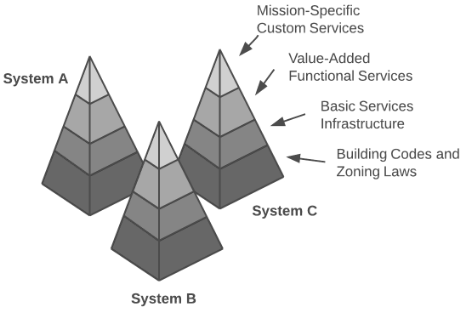
\includegraphics[width=0.4\textwidth]{islandOfAutomation.png}
    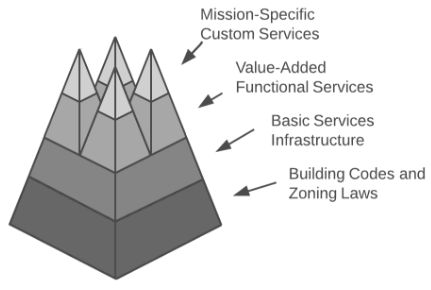
\includegraphics[width=0.4\textwidth]{noIslandOfAutomation.png}

    \footnotesize{(C) SourceMaking.com}

    \tiny{\url{https://sourcemaking.com/antipatterns/stovepipe-enterprise}}
\end{center}

Как бороться с такой ситуацией:

\begin{itemize}
    \item использовать существующие промышленные стандарты. Например, если вся организация работает в сфере робототехники, стандарт де-факто по интеграции компонентов там ROS, так что достаточно мелкие компоненты из разных проектов вполне могут оказаться совместимы и переиспользуемы, а опыт использования ROS как платформы --- переиспользуем.
    \item Фиксировать технологии и типовую архитектуру на уровне предприятия. Это идёт несколько вразрез с тем, что говорилось про <<золотой молоток>>, но если вы берёте только проекты на .NET, сделайте себе репозиторий на всю организацию, положите туда библиотеку переиспользуемых компонентов, настройте NuGet-сервер, создайте шаблоны типовых приложений и т.д.
    \item Вообще, создать и поддерживать инфраструктуру переиспользования. Она может варьироваться от просто корпоративного репозитория с полезным кодом до in-house генераторов типовых приложений или даже предметно-ориентированных визуальных языков (см. опыт Nokia из \url{https://www.metacase.com/cases/nokia.html}). Начальные инвестиции могут быть высоки и это, безусловно, отпугивает, но результирующие преимущества могут быть впечатляющи (тот же опыт Nokia как экстремальный пример, когда in-house-технология позволила нанять неквалифицированных специалистов и дать им возможность производить по одному несложному мобильному приложению в день, что вручную было вообще недосягаемо).
\end{itemize}

\subsection{Stovepipe System}

\noindent\begin{minipage}{\textwidth}
    \begin{minipage}[c][6cm][c]{\dimexpr0.7\textwidth-0.5\Colsep\relax}
        Stovepipe System, <<Система в стиле печной трубы>> --- уточнение Stovepipe Enterprise для отдельной системы, состоящей из компонентов. Характеризуется отсутствием единого стандарта по взаимодействию между подсистемами и интеграцией подсистем по принципу <<как получится>> (<<ad-hoc>>). В этом случае отработанные решения по взаимодействию между компонентами опять-таки не могут помочь друг другу, добавление нового компонента или изменение связей между существующими --- большая работа, а тестирование такой системы --- то ещё удовольствие.
    \end{minipage}\hfill
    \begin{minipage}[c][6cm][c]{\dimexpr0.3\textwidth-0.5\Colsep\relax}
        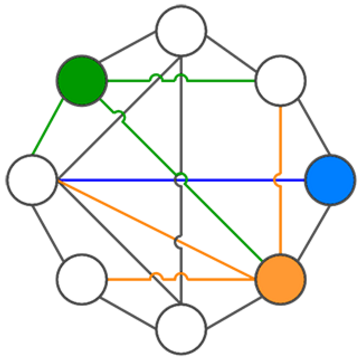
\includegraphics[width=\textwidth]{stovepipeSystem.png}

        \footnotesize{(C) SourceMaking.com}

        \tiny{\url{https://sourcemaking.com/antipatterns/stovepipe-system}}
    \end{minipage}%
\end{minipage}

Как с этим бороться --- как обычно, введением внутренних стандартов. Тут могут помочь и уже существующие стандарты (хороший пример --- тот же ROS, или REST-сервисы), и использование известных паттернов интеграции --- например, Enterprise Service Bus. Более <<тактическое>> решение --- выделение единого интерфейса для подсистем и реализация всего взаимодействия в терминах этого интерфейса (так обычно устроены плагинные системы, например).

\subsection{Vendor Lock−In}

Антипаттерн Vendor Lock−In, или <<зависимость от поставщика>> --- ситуация, когда архитектура вашей системы или её реализация зависит от третьестороннего коммерческого решения, которое вы не можете контролировать. Казалось бы, почему бы не разрабатывать приложение по поддержке электронного обучения HwProj на Ruby, молодой и перспективной технологии? Потому что HwProj используется через семь лет после своего запуска, а Ruby нет --- специалистов, способных поддерживать HwProj, не найти, баги не фиксятся, новые фичи не реализовать. Это весьма типичная ситуация для приложений, у многих из них ужасно долгий жизненный цикл, длящийся десятки лет. Часто приложения надолго переживают технологии, с помощью которых были разработаны. Хороший пример тому --- банковские системы, написанные на COBOL в 80-х годах двадцатого века. Они используются до сих пор, и их слишком опасно и дорого менять, поэтому будут использоваться и дальше, а COBOL помер давно. А сопровождать такие системы надо.

Собственно, долгий жизненный цикл приложений --- не антипаттерн, а суровая реальность. Антипаттерн --- завязываться без нужды на вендора, особенно если нет оснований для уверенности, что он будет поддерживать свою технологию на протяжении ещё хотя бы пары десятилетий. Особенно если эта технология навязывает архитектуру всему приложению и неотделима от полезного кода (например, это платформа, на которой приложение разрабатывается). Если речь идёт про Java, .NET или даже Qt, вряд ли стоит от них отказываться в пользу самодельного компилятора (хотя в критических приложениях типа ОС вооружённых сил --- стоит ещё как!), но если вы пишете приложение на долгие годы вперёд и делаете это на новом хипстерском js-фреймворке известного хипстерского стартапа <<Рога и Копыта>>, то надо принять меры на случай исчезновения фреймворка с рынка.

Какие это могут быть меры:

\begin{itemize}
    \item опять-таки, архитектурная подготовка к изменениям --- микросервисы, просто сервисы, изолированные компоненты;
    \item избегать сильной привязки к подозрительным третьесторонним компонентам --- программировать не <<на>>, а <<с помощью>>;
    \begin{itemize}
        \item интересная тактика по этому поводу используется в некоторых промышленных проектах --- выкладывать в свой репозиторий и компоненту, от которой мы зависим, причём даже в бинарном виде, хоть это и считается табу для систем контроля версий --- пока наш репозиторий жив, зависимости тоже живы; 
        \item более грамотные люди используют Docker-образы для подобных целей;
    \end{itemize}
    \item использовать изоляционный слой --- тонкую прослойку кода между вашей системой и третьесторонним компонентом. Компонент перестали выпускать и вообще убрали из интернета --- не проблема, выкидываем его и заменяем на другой, или пишем свою реализацию, при этом существующий код, кроме изоляционного слоя, менять не надо.
    \item Не бояться реинжиниринга. Если сама платформа, на которой вы писали, померла, может потребоваться выполнить перенос приложения на новую платформу, с использованием методов реинжиниринга типа извлечения бизнес-правил. Это дорого и сложно, но дешевле переписывания с нуля (хотя и само переписывание с нуля в разы дешевле разработки в незнакомой предметной области).
\end{itemize}

\subsection{Architecture By Implication}

Architecture By Implication, или <<неявная архитектура>> --- это антипаттерн архитектуры, отрицающий необходимость явной спецификации архитектуры в случае, если уже есть опыт создания подобных приложений. Фразы-детекторы: <<We’ve done systems like this before!>> и <<There is no risk; we know what we’re doing!>>. Казалось бы, это логично, если опыт есть, есть и типовая архитектура с предыдущего проекта, и технологии, и даже наработки, зачем ещё раз делать одно и то же?

Затем, что требования всё-таки могут различаться, и задачи, кажущиеся похожими, могут содержать в себе скрытые риски, которые при отсутствии явной разработки архитектуры могут остаться незамеченными. Возможно, вы настолько уверены, что задача похожа на предыдущую, что даже не понимаете, что заказчик хочет совсем другого. Плюс к тому, даже если всё хорошо, есть риск <<золотого молотка>>, когда вы снова достаёте проверенную дедовскую технологию, которой сделали уже 20 проектов, и не хотите погуглить новые вещи, которые вашу задачу позволяют решить в разы быстрее и лучше. 

Обратите внимание, переиспользовать архитектурные решения с предыдущих проектов никто не запрещает, причём выработка типовых архитектур и локальной библиотеки паттернов даже очень приветствуется, антипаттерн тут --- отсутствие явной архитектурной документации вообще.

Как с этим бороться --- требовать явного описания архитектуры системы всегда. Можно использовать стандарты Software Design Description (IEEE 1016) или Architecture Description (ISO/IEC 42010), можно (что чаще бывает) выработать свой какой-то внутренний стандарт, но некий диздок должен быть. Можно подойти к этому ещё более структурно и использовать какой-либо архитектурный фреймворк (или просто методологию), где написано, что, когда и как надо создавать, чтобы архитектура считалась нормально описанной. Главное, не оставлять это дело на откуп примерному пониманию программистов.

\subsection{Design By Committee}

Design By Committee, <<проектирование комитетом>> --- попытка принимать архитектурные решения простым большинством голосов (<<A camel is a horse designed by a committee>>). Обсуждать архитектуру большими и шумными компаниями хорошо и правильно, но решения должны либо приниматься единогласно, либо должен быть один человек, который их принимает и отвечает за них. Иначе попытка включить в дизайн идеи, соображения и индивидуальные предпочтения каждого приводит к сложной, объёмной и внутренне противоречивой архитектуре. Хорошие системы вообще дизайнятся одним человеком, либо командой, где есть один главный архитектор, у которого есть видение и идея системы, и помощники, которые либо проектируют отдельные компоненты, либо помогают уточнить дизайн и оформить документацию. Особо опасен этот антипаттерн, когда комитет --- это консорциум из сотни крупных компаний, каждая из которых лоббирует свои интересы и пытается отгрызть долю рынка, <<правильно>> влияя на проект.

Что можно сделать, чтобы избежать этой ситуации --- во-первых, ограничить размер команды. Идеал --- 4 человека, почти идеал --- 6-7 человек (команда, которую <<можно накормить двумя пиццами>>). У Брукса в книжке <<Мифический человеко-месяц>> была интересная идея, что в команде собственно программирует систему только один человек, остальные занимаются вспомогательными задачами (там это называлось <<бригада главного хирурга>>). Такая модель не прижилась, но в любой команде всё равно можно добиться разделения ролей, и надо его строго придерживаться. Должен быть явный главный архитектор, product owner, разработчики, эксперты и т.д. Это всё может быть одно лицо или целые группы, но роли должны быть чётко определены и лицо, принимающее решения, должно быть одно.

\end{document}
